\documentclass[a4 paper,12pt]{article}\usepackage{float, graphicx,xepersian }
\settextfont{Yas}
\setdigitfont{Yas}
\title{درس روش پژوهش و تحقیق دانشجويان علوم كامپيوتر دانشگاه آدلايد استراليا  تهیه : عذرا حسینی دانشگاه پیام نور پردیس }

\date{\today}
\begin{document}
	
\maketitle




\noindent
\vspace{0.1cm}
\vspace{0.1cm}


  \vspace{0.1cm}

\vspace{0.1cm}     
\noindent
این درس ، دانشجویان را برای تحقیقات پیشرفته با بررسی چگونگی برنامه‌ریزی ، اجرا و گزارش درباره تحقیقات تجربی آماده خواهد کرد . این دوره ، تکنیک‌های کاربرد برای هر یک از مراحل یک پروژه تحقیقاتی را پوشش خواهد داد که شامل فرموله کردن سوالات تحقیق ، ایجاد تئوری ، تحلیل داده‌ها ( استفاده از هر دو روش کیفی و کمی ) ، ایجاد مدرک ، ارزیابی اعتبار و انتشار است. این امر به طور خاص بر روی تحقیقات مربوط به نرم‌افزار ، توسعه ابزارهای آماری برای سنجش عملکرد نرم‌افزار و روش‌هایی که در آن افراد با ابزارهای نرم‌افزاری تعامل دارند ، متمرکز خواهد بود\\


كددرس :                  
\lr{COMPSCI7406}          


\vspace{0.1cm}
\vspace{0.1cm}
\vspace{0.1cm}
\noindent
                                                                                           نام درس : روش‌های تحقیق در مهندسی نرم‌افزار و علوم رایانه(كامپيوتر) 

\noindent
زمان ارائه : نيمسال اول تحصيلي \\
سطح : دوره هاي تحصيلات تكميلي\\ 
مكان : پرديس نورت تريس\\
                                                                                                                                                             دو ساعت درهفته تدريس مي شود\\
                                                                                                                                                             سه واحد درسي\\
\noindent   
     شرح درس:  این درس دانشجویان را برای تحقیقات پیشرفته با بررسی چگونگی برنامه‌ریزی , انجام و گزارش تحقیقات تجربی آماده خواهد کرد . این درس تکنیک‌های کاربردی برای هر یک از مراحل یک پروژه تحقیقاتی شامل تدوین سوالات تحقیقاتی , ساخت نظریه , تجزیه و تحلیل داده‌ها ( با استفاده از روش‌های کمی و کیفی ) ساخت مدرک , ارزیابی اعتبار و انتشار را پوشش خواهد داد . تمرکز ویژه بر تحقیق شامل نرم‌افزار , توسعه ابزارهای آماری برای اندازه‌گیری عملکرد نرم‌افزار و روش‌های تعامل افراد با ابزارهای نرم‌افزاری است \\
اساتيد درس : \\
هماهنگ کننده درس : دکتر کریستوفر ترودو \\     
اساتید : دانشیار نیک فالکنرو دکتر کریستوفر ترودو\\
جدول زمانی دوره (درس) :\\

	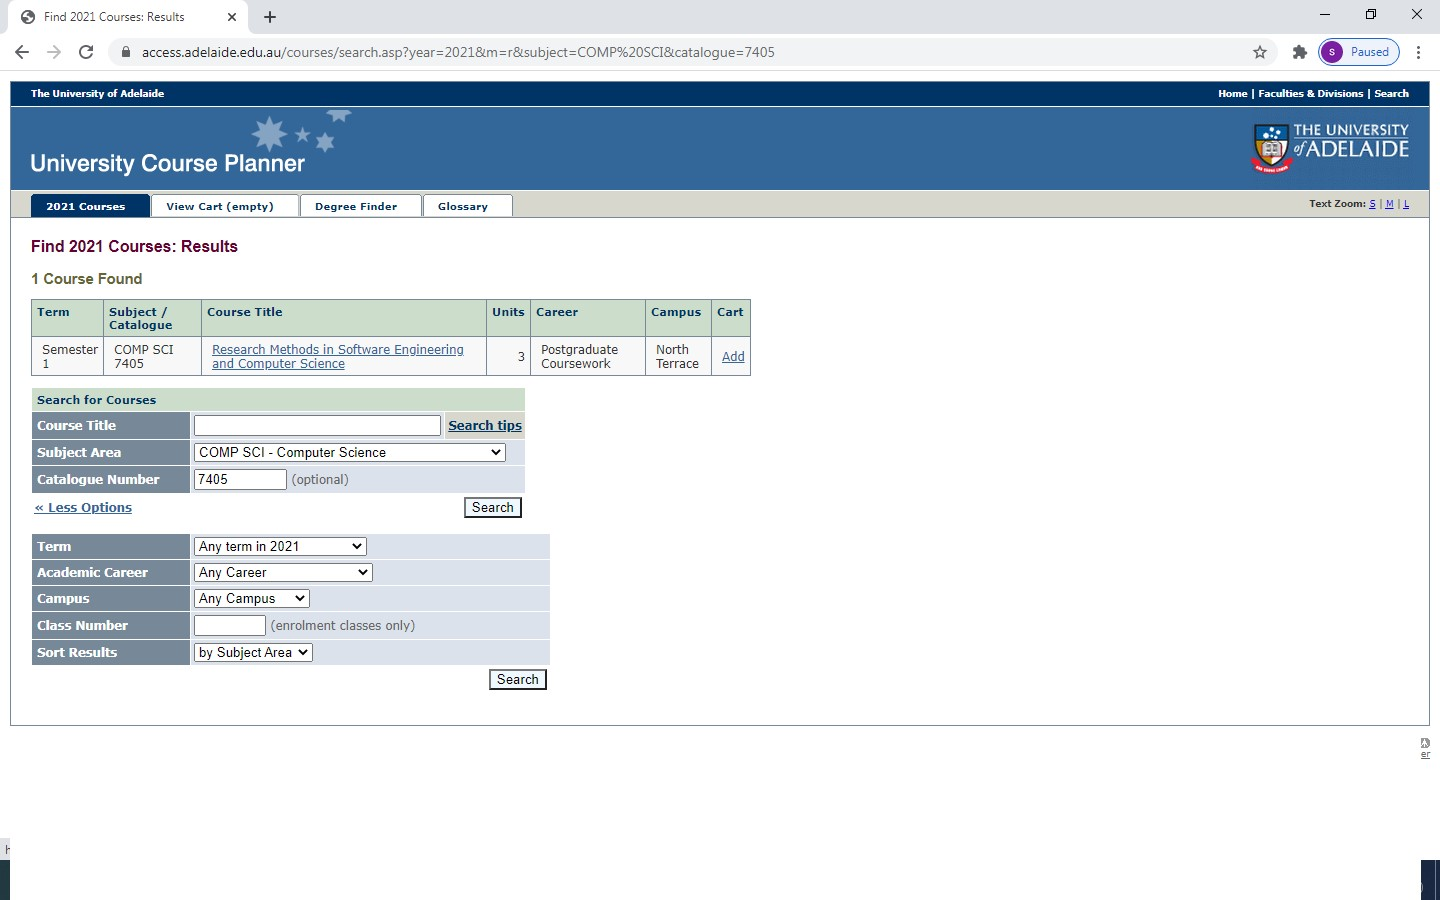
\includegraphics[scale=0.5]{pic1.jpg}

                                                         
                                                     
                                                     
                                                     
                                                     
                                                     
                                                     
                                                                                       \noindent                               
نتایج یادگیری درس :\\
در قبولی موفقیت‌آمیز این درس ، دانشجویان خواهند توانست : \\
1- شناخت و به‌کارگیری فلسفه علم و کاربرد آن در روش‌های تحقیق را یاد خواهند گرفت\\
2- می‌توانند اصول طراحی تحقیق را توضیح دهند\\
3- قادرخواهند بود از اصول طراحی تحقیق برای انواع پروژه‌ها استفاده کنند\\
4- اصول اخلاق پژوهشی و مفاهیم آن را فهمیده و قادر به توضیح آنان خواهند بود\\
5- درک و توانایی استفاده از تکنیک‌هایی از جمله روش‌های کیفی , روش‌های کمی , روش‌های تحقیق , مطالعات موردی , مصاحبه‌ها را دارا خواهند شد\\
6- فهمیدن و توانایی پیداکردن در توضیح مهم تکرارداده ها و مدیریت اداراکی\\
7-   طراحی و اجرای مطالعات تحقیقاتی که نیازمندی‌های بالا را برآورده می‌کنند \\
8- نشان دادن توانایی تولید گزارش‌های مکتوب از کار تحقیقاتی که یک استاندارد بین‌المللی است.\\
9- نشان دادن توانایی نقد و بررسی کار به منظور شناسایی اینکه اصول روش‌شناختی پژوهش به خوبی پی‌گیری شده‌اند یا می‌توانند بهبود یابند , از جمله ارائه مکتوب بازبینی به استاندارد حرفه‌ای \\
نتایج یادگیری دوره بالا با مهندسان استرالیا مرحله ۱ شایستگی برای مهندس حرفه‌ای همخوانی دارد \\
این دوره برای توسعه عناصر زیر طراحی شده‌است .1   1.2   1.3   1.4   1.5   1.6   2.1   2.2   2.3   2.4   3.1   3.2   3.3   3.4   3.5   
ویژگی‌های تحصیلات دانشگاهی\\
این دوره برای ،دانشجویان فرصتی را برای توسعه مشخصه تحصیلات تکمیلی که در زیر مشخص شده‌است ، فراهم می‌کند\\
\\
\\
\\
\\ 
خصوصیات تحصیلات دانشگاهی  /                              نتایج یادگیری دوره\\
\\    ---------------------------------------------------------------------------------
\\
دانش انضباط عمیق\\
در سراسر برنامه تحصیلی خود از تحقیقات لبه برش مطلع شده و آن را القا کرده بودند                                                            9-1\\
تعامل شخصی با مربیان فعال تحقیق ، از سال اول ،\\
معتبر بودن یا تاییدیه داشتن مقابل استانداردهای ملی یا بین‌المللی ( برای برنامه‌های مرتبط )\\
تفکر انتقادی و حل مساله \\
دقت و غرق در روشهای تحقیق                                    7 , 5.9 \\
رویکرد علمی مبتنی بر شواهد تجربی و برای توسعه دانش\\
شان دادن موضوع از طریق ارزیابی مناسب \\
کار گروهی و مهارت‌های ارتباطی                                                                                                                    2,4,9\\
فرم توسعه یافت از طریق روش اس جی دی ای\\
استفاده از ارزیابی و تمرین در طول برنامه مطالعات\\
تشویق و ارزش‌گذاری در تمام جنبه‌های یادگیری\\
\\
آمادگی شغلی و رهبری                                                                                                 3,5,7,9\\
درک و فهم تکنولوژی\\
حرفه‌ای و کاملا ً معتبر\\
فکر کردن و مطلع کردن\\
با تجربیات مبتنی بر کار آزمایشی و تایید شده\\
شایستگی فرهنگی و اخلاقی                                                                                             4\\
\noindent
توانایی فعالیت در فرهنگ‌های دیگر\\
آسوده با ملیت‌های مختلف و بسترهای اجتماعی\\
قادر به تعیین و کمک به پیامدهای اجتماعی مطلوب هستند\\ 
با مطالعه خارج از کشور یا با شناخت دانش‌های بومی \\
خودآگاهی و هوش عاطفی                                                                                                 9-7\\
\noindent
توانایی تفکر و تمایل به مشارکت در ارزیابی خود\\
باز فکرکردن به بازخورد عینی و سازنده سرپرستان و همسالان خود\\
قادر به مذاکره در مورد وضعیت‌های دشوار اجتماعی ، خنثی کردن تعارض و درگیر شدن به طور مثبت در بحث هدفمند هستند \\
منابع یادگیری \\
منابع لازم\\
این دوره هیچ کتاب خواندنی ندارد , امامطالعات در طول درس ارائه می‌شود و ممکن است از طریق پورتال آموزش آنلاین قابل‌دسترسی باشد \\
منابع پیشنهادی\\
منابع پیشنهادی وجود ندارد\\
یادگیری آنلاین\\
سيستم مديريت يادگيري بوم همه مواد درسي از سايت  
\lr{MY Uni}
به آدرس 
\noindent
\lr{Myuni.adelaide.edu.eu}
 قابل دسترسی هستند مواد يادگيري آنلاين به احتمال زياد شامل پادكست ها ضبط ويدئو اسناد الكترونيكي و برگزاري امتحانهاي برخط به منظوربررسي دانش دانشجويان همچنين ممكن است به عنوان بخشي از دوره هاي خود با سيستم پرتفوي مهارا تعامل داشته باشند.  \\
 فعالیت‌های یادگیری و تدریس \\
 روش‌های یادگیری و تدریس \\
 این درس به دانشجویان نیاز دارد تا قبل از شرکت در جلسات به صورت رو به رو ، یک جلسه دو ساعته آماده کنند . صورت رو به رو شامل سخنرانی‌های کوچک ، بحث گروهی ، فعالیت‌های مشارکتی ، ارائه و ارزیابی همکلاسی شان می‌باشد . ضروری است که دانشجویان قبل از شرکت در این جلسه آماده شوند در حالی که جلسات رو به رو ممکن است صبط شوند ، ممکن است این فعالیت‌ها لزوما ً توسط این سیستم ثبت نشوند\\
 
\noindent 
 حجم یا میزان فعالیت وکار\\
 \\
 اطلاعات زیر به عنوان راهنمایی برای کمک به دانش آموزان در تعامل مناسب با الزامات درس ارائه شده‌است 
 انتظار می‌رود که دانشجویان هر هفته با یک جلسه دو ساعته مواجه شوند . فعالیت‌های ارزیابی دوره به طور متوسط چند ساعت در هفته طول خواهد کشید.\\
 از آنجایی که هیچ امتحانی وجود ندارد, فعالیت‌های ارزیابی و حجم کار دانشجویی به 13هفته و احتمالا ً 14 هفته ادامه خواهد یافت\\
 \\
 خلاصه فعالیت‌های یادگیری\\
 این درس دانشجویان را برای تحقیقات پیشرفته با بررسی چگونگی برنامه‌ریزی , انجام و گزارش تحقیقات تجربی آماده خواهد کرد . این درس تکنیک‌های کاربردی برای هر یک از مراحل یک پروژه تحقیقاتی شامل تدوین سوالات تحقیقاتی , ساخت نظریه , تجزیه و تحلیل داده‌ها ( با استفاده از روش‌های کمی و کیفی ) , ساخت مدرک , ارزیابی اعتبار و انتشار را پوشش خواهد داد . تمرکز ویژه بر تحقیق شامل نرم‌افزار , توسعه ابزارهای آماری برای اندازه‌گیری عملکرد نرم‌افزار و روش‌های تعامل افراد با ابزارهای نرم‌افزاری است. \\
 الزامات دوره خاص\\
 دانشجویان باید سال آخر یک دوره کارشناسی باشند , که در یک برنامه آموزشی ممتاز ثبت‌نام کرده‌اند یا برنامه دکترا را آغاز کرده‌اند. ترجیحا ً، دانشجویان باید کار پروژه خود را آغاز کنند و بتوانند این دوره را در رابطه با ۶ تا ۱۲ ماه اول پروژه خود انجام دهند\\
 
\noindent 
 تجربه کشف کردن گروه کوچک\\
 تمرکز این درس , تحقیق و دانشجویان برای انجام فعالیت‌های گروهی کوچک به عنوان بخشی از دوره است. \\
 ارزیابی\\
 سیاست دانشگاه درباره ارزیابی برنامه‌های آموزشی براساس چهار اصل زیر است: \\
 1- ارزیابی باید مشوق و تقویت یادگیری باشد\\
 2- ارزیابی باید به قضاوت قوی و منصفانه درباره عملکرد دانشجویان کمک کند\\ 
 3- روش‌های ارزیابی باید عادلانه و برابر باشند و به دانشجویان فرصت نشان دادن آنچه را که آموخته‌اند بدهند \\
 4- ارزیابی باید استانداردهای آکادمیک را حفظ کند \\
 خلاصه ارزیابی \\
 	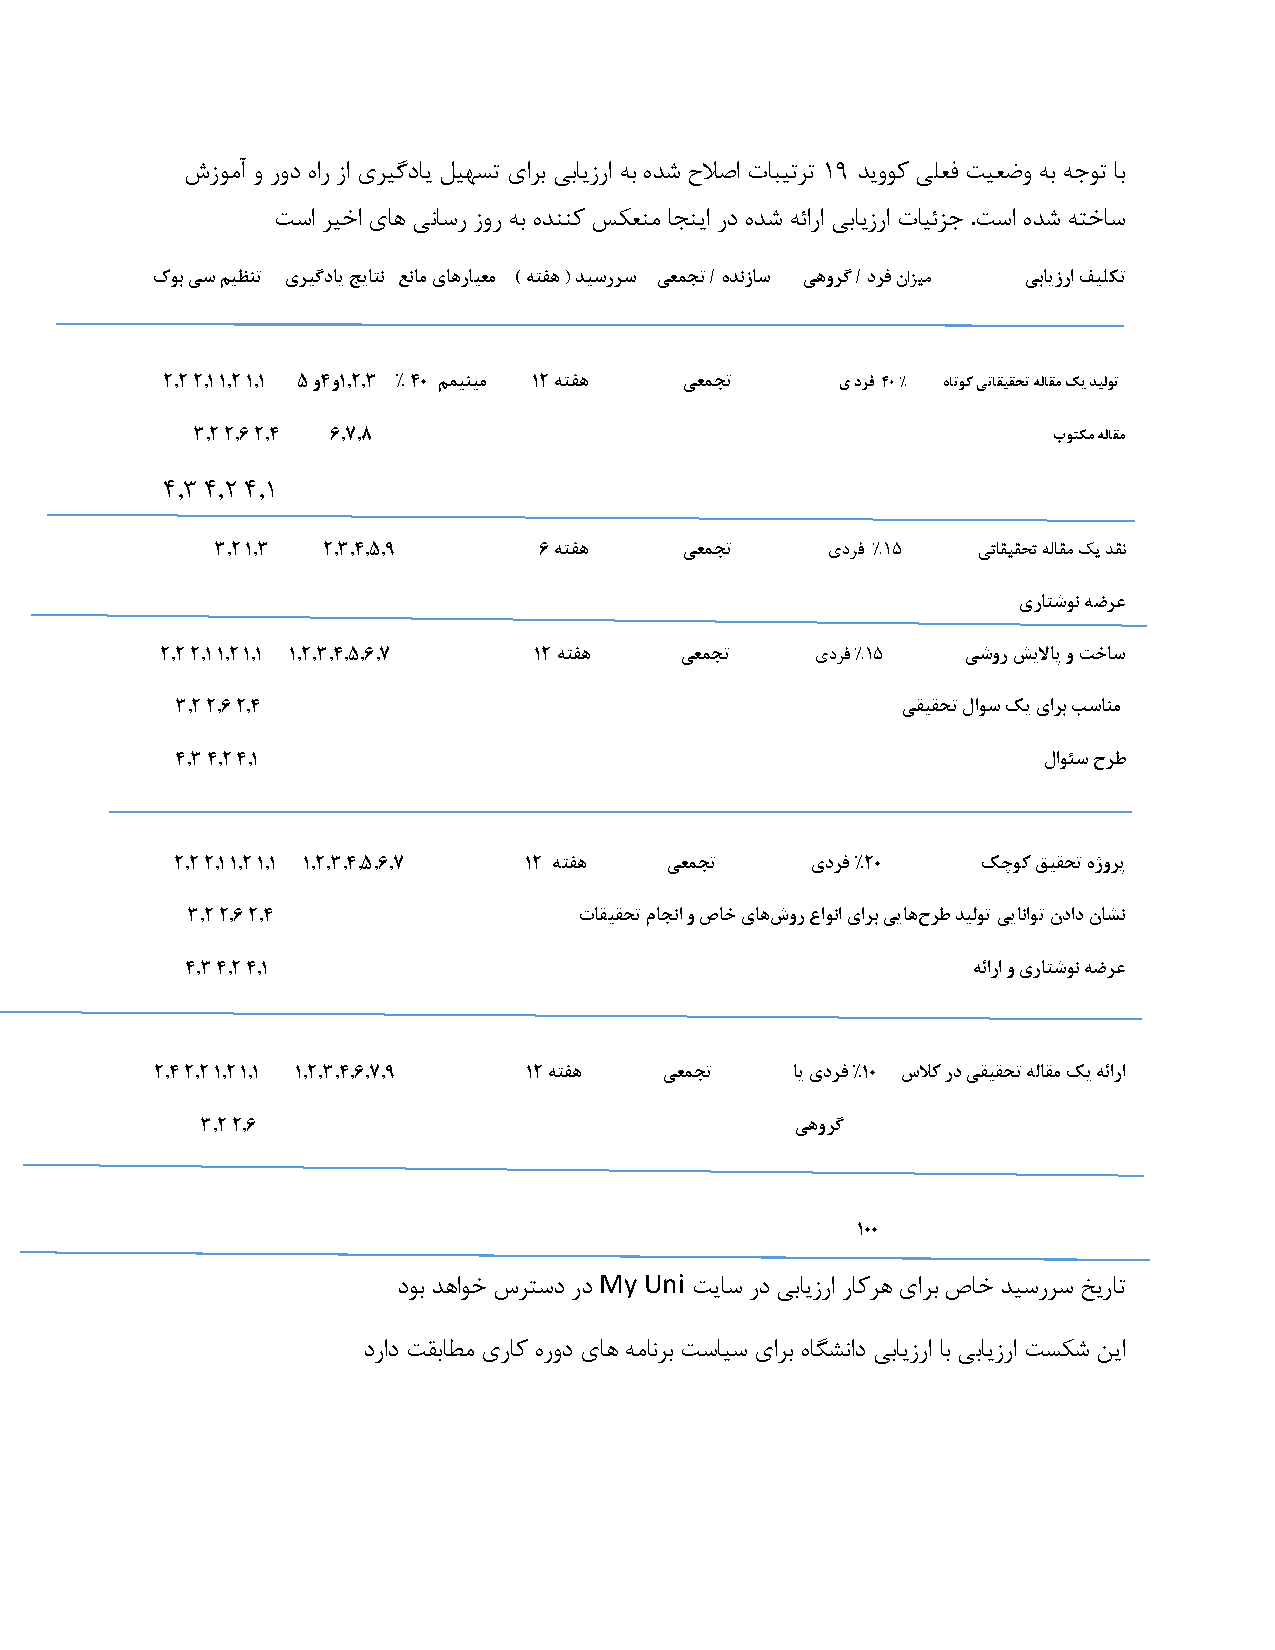
\includegraphics[scale=0.45]{arz.pdf}
\begin{latin} 	 
\noindent	
 CBOK is the Core Body of Knowledge for ICT Professionals defined by the Australian Computer Society . The alignment in the table above corresponds with the following CBOK Areas
 \end{latin}
\noindent
سي بوك هسته مرکزی دانش متخصصان فاوا است که توسط جامعه کامپیوتر استرالیا تعریف شده‌است. همترازی در جدول بالا مربوط به حوزه‌های زیر است \\
:1- حل مساله\\
1.1 چكيده\\
1.2 طراحي\\
2- دانش حرفه‌ای\\
2.1 اصول\\
2.2 انتظارات حرفه‌ای\\
2.3 مفاهیم و موضوعات کار گروهی\\
2.4 ارتباطات بین فردی\\
2.5 مسائل اجتماعی\\
2.6آشنايي با حرفه 
\lr{ICT}
\\
3- منابع تکنولوژی \\
3.2 داده و اطلاعات\\
3.3شبكه\\
4- ساختمان تکنولوژی\\
4.1 برنامه نويسي\\
4.2 عوامل انسانی\\
4.3 توسعه سیستم‌ها\\
4.4 فراگيري سیستم‌ها

\noindent
5- مديريت 
\lr{ICT}\\
\noindent
5.1 حاکمیت و سازمان  
\lr{IT}\\
\noindent
5.2 مدیریت پروژه    
\lr{IT}\\
\noindent
5.3 مدیریت خدمت\\
5.4 مدیریت امنیت\\

\noindent
ارزیابی الزامات مرتبط\\

\noindent
شرط مانع : اگر نمره کلی شما برای این درس بیشتر از اف 44باشد اما , نمره شما برای مقاله تحقیقات کوتاه کم‌تر از 40 درصد باشد نمره كلي شما برای این درس به اف 44 كاهش پيدا مي كند 

\noindent   
   جزئیات ارزیابی  \\
   \\
   تجزیه و تحلیل دقیق ارزیابی این است:\\
   1- فراهم كردن مقاله کوتاه تحقیقي . مقاله نوشته شده .40 درصد\\
   2- نقد یک مقاله تحقیقاتی . عرضه و ارائه کتبی  15درصد\\
   3- ساختن یک روش مناسب برای یک سوال پژوهشی عرضه نوشتاری 15 درصد\\
   4 - پروژه تحقیقاتی كوچك : توانایی تولید طرح‌ها برای طیف وسیعی از روش‌های خاص را نشان دهید و تحقیقات را انجام دهید ارائه وعرضه کتبی 20 درصد\\
   5- ارائه در کلاس 10 درصد(درجه بندی شده توسط مدرس و ارزیابی هم تیم پروژه دو ارائه جداگانه مربوط به پروژه)\\
      مورد ۱ الزام دشواری برای این دوره است . دانشجويان باید حداقل ۴۰  درصداز نمره در دسترس برای این بخش را داشته باشند \\
\noindent
\\      
   تهیه نقشه سي بوك\\
   \\
\noindent   
   مقاله تحقیقاتی\\
   \\
   چكيده 3\\
   طراحي 3 \\
   اخلاق  3\\
   انتظارات حرفه‌ای  2 \\
   ارتباطات بین فردی 3 \\
   آشنایی با حرفه
\lr{ICT}3\\
\noindent
داده و اطلاعات 3\\
برنامه نويسي 3 \\
عوامل انسانی3  \\
توسعه سیستم‌ها 3 \\
\\
نقد \\
\\
اخلاق 4 \\
داده و اطلاعات 4  \\

\noindent
ساخت و پالایش روش \\
\\
چكيده 3 \\
طراحي  3 \\
اخلاق  3  \\
انتظارات حرفه‌ای 2 \\
ارتباطات بین فردی 3\\
آشنایی با حرفه
\lr{ICT}3\\
داده و اطلاعات3  \\
برنامه نويسي 3\\
عوامل انسانی3  \\
توسعه سیستم‌ها 3\\


\noindent
پروژه تحقيق كوچك \\
\noindent
طراحي 3\\
اخلاق  3\\
انتظارات حرفه‌ای2 \\
ارتباطات بین فردی 3 \\
آشنایی با حرفه
\lr{ICT}3\\
برنامه نويسي  3\\
عوامل انسانی3 \\ 
توسعه سیستم‌ها 3\\
\\
\noindent
ارائه يك مقاله تحقيقاتي \\
\\
اخلاق 3\\
انتظارات حرفه‌ای2 \\
ارتباطات بین فردی 3 \\
آشنایی با حرفه
\lr{ICT}\\
داده و اطلاعات 3\\
عرضه\\
\\
\noindent
تمام کارها از طریق دروازه ارسال وب علوم کامپیوترال ام اس و یا مهارا سیستم پورتفولیوی پروژه انجام خواهد شد  هرانتساب وضوح دستورها نسبت به حالت ارسال و مدل مدیریت تاخیر دارد که مورد استفاده قرار می‌گیرد 
در این کلاس خطاهاي سنتی ممکن است مورد استفاده قرار نگیرد ، اگر چه در غیر این صورت ، این مدلی است که مورد استفاده قرار خواهد گرفت . در عوض ، هنگامی که به وضوح مشخص شد ، ارائه دیر هنگام ممکن است منجر به از دست دادن دسترسی به منابع درجه بندي خاص شود . ( به عنوان مثال ، دلایل مستند برای تاخیر می‌تواند قابل‌قبول باشد و ما در صورتی که کار در زمانی که برای مرور هم پروژ ه اي توزیع نشده باشد ارائه نگردد ، این کار علامت بازبینی هم پروژ ه اي را دریافت نخواهد کرد . اگر کار در زمان برای علامت‌گذاری مفصل انجام نشود ، یک موضوع ساده‌تر به کار گرفته خواهد شد که زمانی که تمام نشانه‌های دیگر ارسالی تکمیل شده‌باشد و اگر زمان اجازه ‌دهد و فرصتهاي کمتری برای دریافت نشانه‌ها داشته باشد و اگر یک دانشجو برای ارائه خود آمادگی نداشته باشد ، این امتیاز از دست می‌رود.
\\
درجه بندی دوره(درس)\\
نمرات عملکرد شما در این درس طبق طرح زیر اعطا می‌شود: \\
	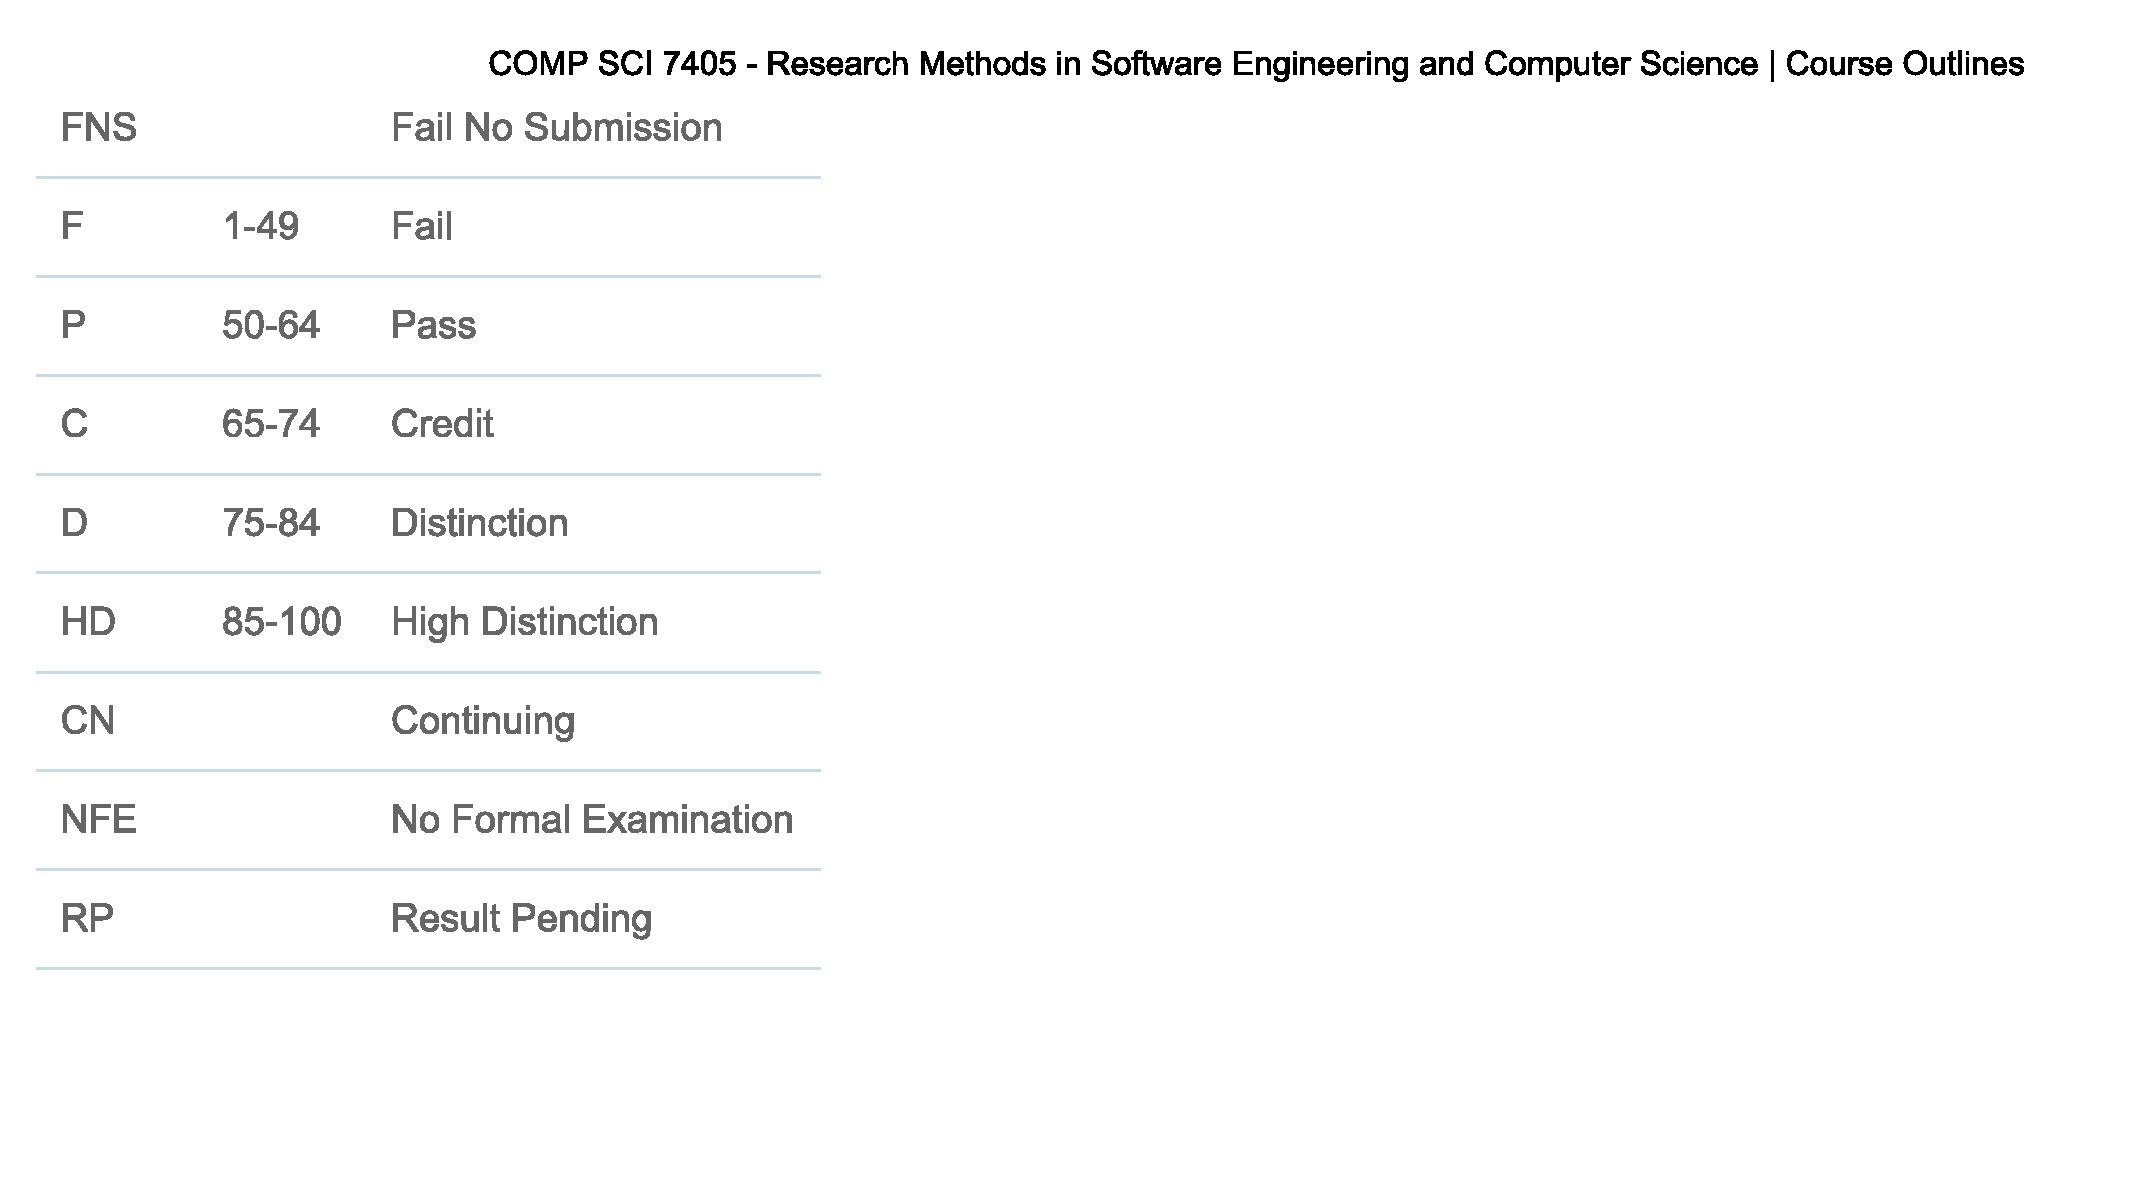
\includegraphics[scale=0.37]{pic2.jpg}
\noindent
جزییات بیشتر نمرات / نتایج را می‌توان از آزمون‌ها به دست آورد. \\ 
توصیف‌کننده‌های درجه در دسترس هستند که راهنمای کلی برای استاندارد کاری هستند که در هر سطح کلاس انتظار می‌رود. اطلاعات بیشتر در مورد ارزيابي برنامه ها در\\
\lr{Assessment for Coursework Programs} \\
\noindent
نتایج نهایی این درس از طریق سایت زیر قابل دسترسی می باشد\\
\lr{Access Adelaide} \\

\end{document}



\end{document}

